%-------------------------------------------------------------------------------
%	PAQUETES Y OTRAS CONFIGURACIONES
%-------------------------------------------------------------------------------

%----------------------------------------------------------------------------------------
%	PAQUETES Y OTRAS CONFIGURACIONES
%----------------------------------------------------------------------------------------

\documentclass[paper=letter, fontsize=11pt]{scrartcl} % Tamaño de papel y letra para el documento

\usepackage[utf8]{inputenc} % Los caracteres acentuados se pueden escribir normalmente en el código
\usepackage[T1]{fontenc} % Configuración de fuente de salida
\usepackage{fourier} % Se usa una fuente diferente al default
\usepackage[spanish,es-noquoting]{babel} % Se configura como documento en español
\usepackage{amsmath,amsfonts,amsthm} % Paquetes para escribir formulas matemáticas
\usepackage{graphicx} % Paquetes para incluir imágenes

\usepackage{circuitikz}
\usepackage{tikz}
\usetikzlibrary{arrows}

\usepackage{sectsty} % Paquete para configuración de secciones
\allsectionsfont{\centering \normalfont \scshape} % Los títulos de las secciones son centrados, con la misma fuente y pequeñas mayúsculas

\usepackage{todonotes}
\usepackage{microtype}

\usepackage{fancyhdr} % Paquete para personalizar pies y cabeceras de página
\pagestyle{fancyplain} % Todas las páginas con las mismas cabeceras y pies de página
\fancyhead{} % Sin cabecera
\fancyfoot[L]{} % Vacío en la izquierda del pie de página
\fancyfoot[C]{} % Vacío en el centro del pie de página
\fancyfoot[R]{\thepage} % Número de página en el pie de pagina
\renewcommand{\headrulewidth}{0pt} % Sin lineas en la cabecera
\renewcommand{\footrulewidth}{0pt} % Sin lineas en el pie de página
\setlength{\headheight}{13.6pt} % Altura de cabecera

\numberwithin{equation}{section} % Numera ecuaciones en cada sección
\numberwithin{figure}{section} % Numera figuras en cada sección
\numberwithin{table}{section} % Numera tablas en cada sección

\setlength\parindent{0pt} % Quita la indentación de los párrafos

\newcommand{\horrule}[1]{\rule{\linewidth}{#1}} % Comando personalizado para hacer linea horizontal


%-------------------------------------------------------------------------------
%	TITULO
%-------------------------------------------------------------------------------

\title{
	\normalfont \normalsize
	\begin{figure}[h]
		\begin{center}
			
\includegraphics[width=0.3\textwidth]{../images/UNITEC.png} % La imagen esta incluida en el mismo directorio del código
		\end{center}
	\end{figure}
	\textsc{Instrumentación y Control} \\ [25pt]
	\horrule{0.5pt} \\[0.4cm] % Linea horizontal delgada
	\huge Práctica 6 - Sistema de Control PID \\ % Titulo de la práctica
	\horrule{2pt} \\[0.5cm] % Linea horizontal mas gruesa
}

\author{Roberto Cadena Vega} % Nombre del profesor

\date{\normalsize 24 de julio de 2014} % Fecha de la práctica

%-------------------------------------------------------------------------------
%	EMPIEZA EL DOCUMENTO
%-------------------------------------------------------------------------------

\begin{document}

\maketitle % Imprime el título

%-------------------------------------------------------------------------------
%	OBJETIVOS
%-------------------------------------------------------------------------------

\section{Objetivos}

	Implementar un sistema de control automático de tipo PID.

%-------------------------------------------------------------------------------
%	CONOCIMIENTOS PREVIOS
%-------------------------------------------------------------------------------

\section{Conocimientos Previos}

%-------------------------------------------------------------------------------

	\subsection{Control PID}

		Un sistema de control tiene 3 componentes importantes:

%-------------------------------------------------------------------------------

		\subsubsection{Control P}

			El control Proporcional no es más que una ganancia:

			\begin{center}
				\tikzstyle{input} = [coordinate]
				\tikzstyle{output} = [coordinate]
				\tikzstyle{block} = [draw, rectangle, minimum height=3em, minimum width=6em]
				\tikzstyle{init} = [pin edge={to-, thin, black}]

				\begin{tikzpicture}[auto, node distance=3cm, >=latex']
					\node [input, name=entrada] {};
					\node [block, right of=entrada] (amplificador) {$k_P$};
					\node [output, right of=amplificador] (salida) {};

					\draw [->] (entrada) -- node[name=x] {$x$} (amplificador);
					\draw [->] (amplificador) -- node[name=y] {$y$} (salida);
				\end{tikzpicture}
			\end{center}

			por lo que lo podemos ver simplemente como el siguiente circuito eléctrico:

			\begin{center}
				\begin{circuitikz} \draw
					(0,0) node[op amp](opamp){}
					(opamp.+) to [R, l=$R_I$] (-4, -0.5) to [short, -o] (-4, -0.5) node[left] {$x$}
					(opamp.-) to [short, *-] (-2, 0.5) to [R, l=$R_I$] (-5, 0.5) node[ground] {}
					(opamp.-) to [short, *-] (-1.2, 2) to [R, l=$R_f$] (1.2, 2)
					(opamp.out) to [short, *-o] (2, 0) node[right] {$y$}
					(opamp.out) to [short, *-] (1.2, 2)
					(opamp.down) node[ground] {}
					(opamp.up) to [short, -o] (-0.08, 1) node[above] {$V_+$}
				;\end{circuitikz}
			\end{center}

			de donde podemos podemos inferir que:

			\begin{equation}
				k_P = \frac{R_f}{R_I} + 1
			\end{equation}

			Por lo que un control P, lo podemos diseñar encontrando las resistencias correctas para la ganancia deseada.

%-------------------------------------------------------------------------------

		\subsubsection{Control I}

			El control Integral es una ganancia con un integrador:

			\begin{center}
				\tikzstyle{input} = [coordinate]
				\tikzstyle{output} = [coordinate]
				\tikzstyle{block} = [draw, rectangle, minimum height=3em, minimum width=6em]
				\tikzstyle{init} = [pin edge={to-, thin, black}]

				\begin{tikzpicture}[auto, node distance=3cm, >=latex']
					\node [input, name=entrada] {};
					\node [block, right of=entrada] (amplificador) {$\frac{k_I}{s}$};
					\node [output, right of=amplificador] (salida) {};

					\draw [->] (entrada) -- node[name=x] {$x$} (amplificador);
					\draw [->] (amplificador) -- node[name=y] {$y$} (salida);
				\end{tikzpicture}
			\end{center}

			el cual podemos construir con el siguiente circuito eléctrico:

			\begin{center}
				\begin{circuitikz} \draw
					(0,0) node[op amp](opamp){}
					(opamp.+) to [R, l=$R$] (-4, -0.5) node[ground] {}
					(opamp.-) to [short, *-] (-2, 0.5) to [R, l=$R$] (-5, 0.5) node[left] {$x$}
					(opamp.-) to [short, *-] (-1.2, 2) to [C, l=$C$] (1.2, 2)
					(opamp.out) to [short, *-o] (2, 0) node[right] {$y$}
					(opamp.out) to [short, *-] (1.2, 2)
					(opamp.down) node[ground] {}
					(opamp.up) to [short, -o] (-0.08, 1) node[above] {$V_+$}
				;\end{circuitikz}
			\end{center}

			de donde podemos podemos inferir que:

			\begin{equation}
				k_I = - \frac{1}{RC}
			\end{equation}

			Por lo que un control I, lo podemos diseñar encontrando la resistencia y el capacitor correcto para la ganancia $k_I$ deseada.

%-------------------------------------------------------------------------------

		\subsubsection{Control D}

			El control Derivativo es una ganancia con un derivador:

			\begin{center}
				\tikzstyle{input} = [coordinate]
				\tikzstyle{output} = [coordinate]
				\tikzstyle{block} = [draw, rectangle, minimum height=3em, minimum width=6em]
				\tikzstyle{init} = [pin edge={to-, thin, black}]

				\begin{tikzpicture}[auto, node distance=3cm, >=latex']
					\node [input, name=entrada] {};
					\node [block, right of=entrada] (amplificador) {$k_D s$};
					\node [output, right of=amplificador] (salida) {};

					\draw [->] (entrada) -- node[name=x] {$x$} (amplificador);
					\draw [->] (amplificador) -- node[name=y] {$y$} (salida);
				\end{tikzpicture}
			\end{center}

			el cual podemos construir con el siguiente circuito eléctrico:

			\begin{center}
				\begin{circuitikz} \draw
					(0,0) node[op amp](opamp){}
					(opamp.+) to [R, l=$R$] (-4, -0.5) node[ground] {}
					(opamp.-) to [short, *-] (-2, 0.5) to [C, l=$C$] (-5, 0.5) node[left] {$x$}
					(opamp.-) to [short, *-] (-1.2, 2) to [R, l=$R$] (1.2, 2)
					(opamp.out) to [short, *-o] (2, 0) node[right] {$y$}
					(opamp.out) to [short, *-] (1.2, 2)
					(opamp.down) node[ground] {}
					(opamp.up) to [short, -o] (-0.08, 1) node[above] {$V_+$}
				;\end{circuitikz}
			\end{center}

			de donde podemos podemos inferir que:

			\begin{equation}
				k_D = - RC
			\end{equation}

			Por lo que un control D, lo podemos diseñar encontrando la resistencia y el capacitor correcto para la ganancia $k_D$ deseada.

%-------------------------------------------------------------------------------

	\subsection{Implementación práctica}

		En la práctica un controlador PID completamente analógico tiene diversas desventajas, por lo que la implementación que utilizaremos es digital (y más cercana a las usadas en la industria.)

		El profesor te proporcionará el siguiente circuito:

		\begin{figure}[h]
			\begin{center}
				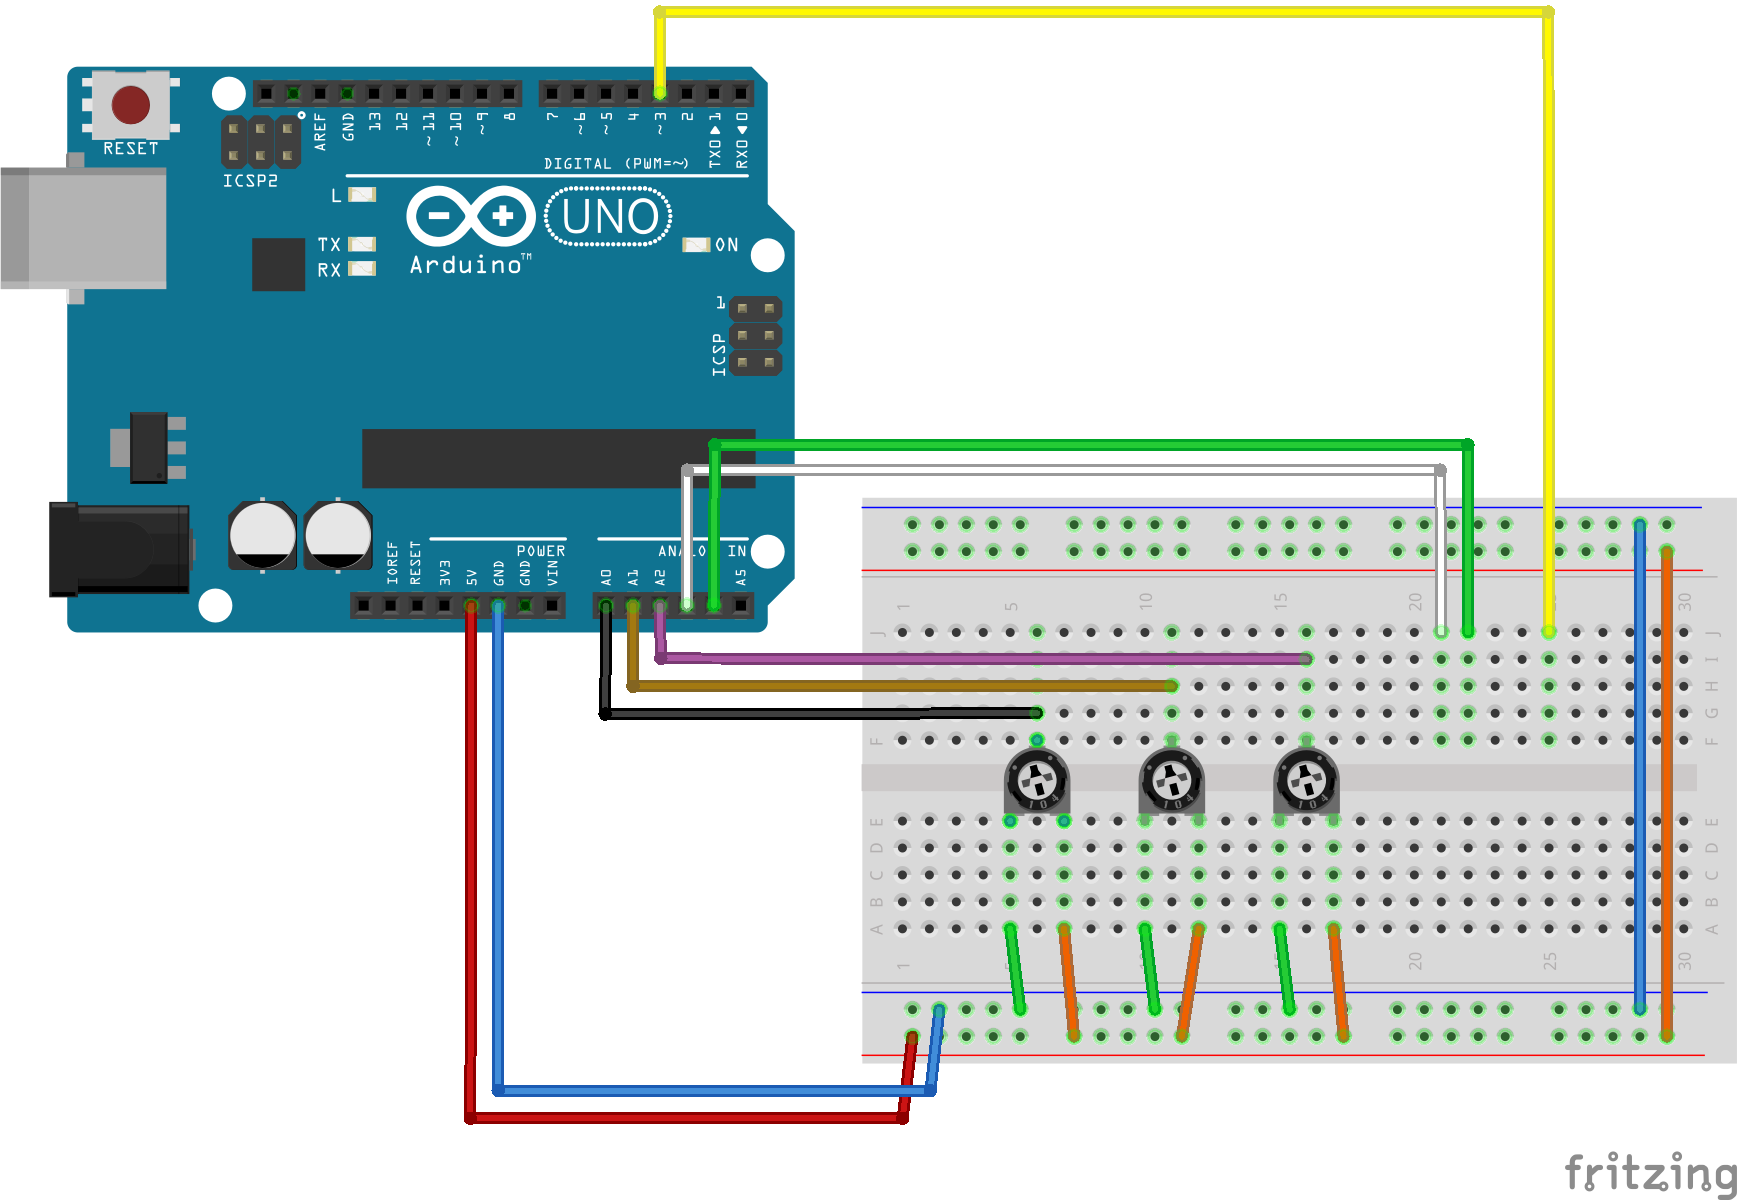
\includegraphics[width=0.5\textwidth]{images/ControlPID.png}
			\end{center}
		\end{figure}

		En el que se toma la señal de tres potenciómetros para calibrar las ganancias $k_P$, $k_I$ y $k_D$ y el programa en el microcontrolador calcula la señal que debe de entregar. La parte importante del código es la siguiente:

		\begin{verbatim}
			// Calculo de error
			error = referencia - entrada;
			// y de la integral del error
			integral = integral + error;

			// Calculo de salida del controlador
			salida = kp*error + kd*(error - error_anterior) + ki*integral;
			if (salida < 0.0 ) {
				salida = 0.0;
			}
			// Se guarda el valor del error en una variable global
			error_anterior = error;
		\end{verbatim}

		Este código utiliza básicamente la siguiente ecuación:

		\begin{equation}
			V_O = k_P V_I + k_d \frac{d V_I}{dt} + k_I \int_0^t V_I dt
		\end{equation}

		Puedes revisar el código completo en el repositorio de la clase; pero por ahora es suficiente con decir, que la entrada de la señal de referencia es el pin A3, la señal del sensor debe entrar en el pin A4. A0, A1 y A2 leen las ganancias P, I y D y la salida de la señal está en el pin 3.
%-------------------------------------------------------------------------------
%	EQUIPO
%-------------------------------------------------------------------------------

\section{Equipo}

	El siguiente equipo será proporcionado por el laboratorio, siempre y cuando lleguen en los primeros 15 minutos de la práctica, y hagan el vale conteniendo el siguiente equipo (exceptuando las pinzas).

	\begin{itemize}
		\item 1 Fuente de Alimentación
		\item 1 Multímetro
		\item 1 Osciloscopio
		\item 1 Generador de funciones
		\item 3 Cable de alimentación
		\item 2 Cables banana - caimán
		\item 2 Cables coaxial - caimán
		\item Pinzas
	\end{itemize}

%-------------------------------------------------------------------------------
%	MATERIALES
%-------------------------------------------------------------------------------

\section{Materiales}

	\begin{itemize}
		\item Protoboard
		\item 1 LED
		\item 1 Potenciómetro $10 k\Omega$
		\item Resistencias
		\begin{itemize}
			\item $180 \Omega$
			\item $220 \Omega$
			\item $330 \Omega$
			\item $470 \Omega$
			\item $1 k\Omega$
			\item $2.2 k\Omega$
			\item $3.3 k\Omega$
			\item $4.7 k\Omega$
			\item $10 k\Omega$
		\end{itemize}
		\item Cables
	\end{itemize}

%-------------------------------------------------------------------------------
%	DESARROLLO
%-------------------------------------------------------------------------------

\section{Desarrollo}

	\begin{enumerate}
		\item Diseña un circuito con un LED, que se pueda acoplar a un sistema de control PID suministrado por el profesor; utiliza una fotorresistencia para darle la señal de retroalimentación a tu controlador y diseña un divisor de voltaje con un potenciómetro, o con un par de resistencias que te dé la señal de referencia.
		\item Sintoniza el controlador por medio de las reglas de sintonización de Ziegler - Nichols.
	\end{enumerate}

%-------------------------------------------------------------------------------
%	CONCLUSIONES
%-------------------------------------------------------------------------------

\section{Conclusiones}

	El alumno deberá describir sus conclusiones al final de su reporte de práctica.

%-------------------------------------------------------------------------------
%	CUESTIONARIO
%-------------------------------------------------------------------------------

\clearpage
\section{Cuestionario - Práctica 6}
	Nombre del alumno: \\[0.2cm]
	\horrule{0.5pt} \\[0.2cm] % Linea horizontal delgada

	\begin{enumerate}
		\item ¿Bastaría con conectar un interruptor para implementar un sistema de control PID? \\ \\ \\ \\
		\item ¿Cuántos métodos de sintonización llevan el nombre Ziegler - Nichols? \\ \\ \\ \\
		\item Si se desea realizar un divisor de voltaje que me dé como voltaje de salida $2.5 V$, y tenga como entrada $5 V$ ¿Qué resistencias se deberán utilizar? \\ \\ \\ \\
		\item Diseña un circuito eléctrico para un controlador P, que debe tener una ganancia $k_P = 15$. \\ \\ \\ \\
		\item Diseña un circuito eléctrico para un controlador PI, que debe tener las ganancias $k_P = 10$ y $k_I = 8$. \\
	\end{enumerate}

%-------------------------------------------------------------------------------
%	HOJA DE ANOTACIONES
%-------------------------------------------------------------------------------

\clearpage
\section{Hoja de Anotaciones}

	\begin{enumerate}
		\item Dibuja el diagrama de conexiones para tu circuito y el diagrama de bloques de tu sistema. \newline \newline \newline \newline \newline \newline \newline \newline \newline \newline \newline \newline \newline \newline \newline \newline \newline \newline \newline \newline \newline \newline \newline \newline \newline \newline \newline \newline
	\end{enumerate}

	Integrantes del equipo: \\[0.2cm]
	\horrule{0.5pt} \\[0.2cm] % Linea horizontal delgada
	\horrule{0.5pt} \\[0.2cm] % Linea horizontal delgada
	\horrule{0.5pt} \\[0.2cm] % Linea horizontal delgada
	\horrule{0.5pt} % Linea horizontal delgada

	Revisó: \\[0.2cm]
	\horrule{0.5pt} \\% Linea horizontal delgada

%-------------------------------------------------------------------------------
%	FIN DEL DOCUMENTO
%-------------------------------------------------------------------------------

\end{document}
